\documentclass{article}
\usepackage{amsfonts, amsbsy, amssymb, amsmath, graphicx, float, subfigure}

\tolerance=5000 
\textwidth=16.6 cm 
\oddsidemargin=-.04 cm
\evensidemargin=-.04 cm 
\topmargin=-1.3 cm 
\textheight=22.9 cm




\newtheorem{definition}{Definition}
\newtheorem{assumption}{Assumption}
\newtheorem{hyp}{Hypothesis}
\newtheorem{theorem}{Theorem}
\newtheorem{lemma}{Lemma}[section]
\newtheorem{corollary}{Corollary}[section]
\newtheorem{proposition}{Proposition}[section]



\begin{document}






\section*{One Degree-of-Freedom (DoF) Hamiltonian Bifurcation of Equilibria}

We will now consider two examples of bifurcation of equilibria in two dimensional Hamiltonian system; in particular, the Hamiltonian saddle-node and Hamiltonian pitchfork bifurcations.  

\subsection*{Hamiltonian saddle-node bifurcation}

We consider the Hamiltonian:

\begin{equation}
H (q, p) = \frac{p^2}{2} - \lambda q + \frac{q^3}{3}, \quad (q, p) \in \mathbb{R}^2.
\label{eq:hamApp13}
\end{equation}

\noindent
where $\lambda$ is considered to be a parameter that can be varied. From this Hamiltonian, we derive Hamilton's equations:

\begin{eqnarray}
\dot{q} & = & \frac{\partial H}{\partial p} = p, \nonumber \\
\dot{p} & = & -\frac{\partial H}{\partial q} =\lambda - q^2.
\label{eq:hamApp14}
\end{eqnarray}

\noindent
The fixed points for \eqref{eq:hamApp14} are:

\begin{equation}
(q, p) = (\pm\sqrt{\lambda}, 0),
\end{equation}

\noindent
from which it follows that there are no fixed points for $\lambda <0$, one fixed point for $\lambda =0$, and  two fixed points for $\lambda >0$. This is the scenario for a saddle-node bifurcation. 

Next we examine stability of the fixed points. The Jacobian of \eqref{eq:hamApp14} is given by:

\begin{equation}
\left(
\begin{array}{cc} 
0 & 1\\
-2 q & 0
\end{array}
\right).
\label{eq:hamApp15}
\end{equation}

\noindent
The eigenvalues of this matrix are:

\[
\lambda_{1, 2} = \pm \sqrt{-2q}.
\]

\noindent
Hence $(q, p) = (-\sqrt{\lambda}, 0)$ is a saddle, $(q, p) = (\sqrt{\lambda}, 0)$ is a center, and $(q, p) = (0, 0)$  has two zero eigenvalues. The phase portraits are shown in Fig. \ref{fig:appC_fig3}.




 \begin{figure}[htb!]
\begin{center}
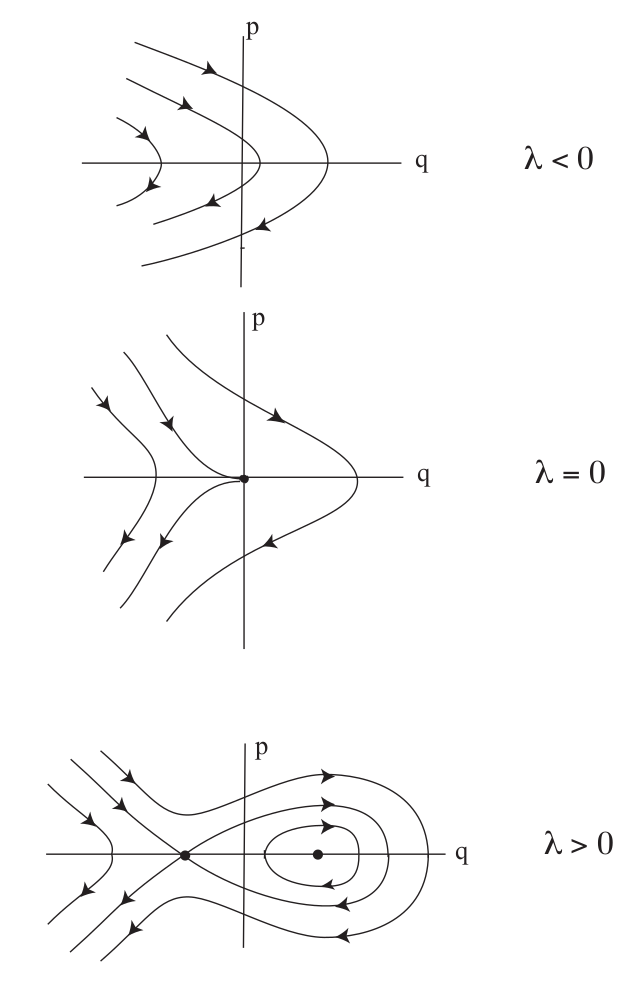
\includegraphics[width=0.6\columnwidth]{ham_sn.png}
\end{center}
\caption{The phase portraits for the Hamiltonian saddle-node bifurcation.}
\label{fig:appC_fig3}
\end{figure}




\subsection*{Hamiltonian pitchfork bifurcation}

We consider the Hamiltonian:

\begin{equation}
H (q, p) = \frac{p^2}{2} - \lambda \frac{q^2}{2} + \frac{q^4}{4},
\label{eq:hamApp16}
\end{equation}

\noindent
where $\lambda$ is considered to be a parameter that can be varied. From this Hamiltonian, we derive Hamilton's equations:

\begin{eqnarray}
\dot{q} & = & \frac{\partial H}{\partial p} = p, \nonumber \\
\dot{p} & = & -\frac{\partial H}{\partial q} =\lambda q  -  q^3.
\label{eq:hamApp17}
\end{eqnarray}

\noindent
The fixed points for \eqref{eq:hamApp17} are:

\begin{equation}
(q, p) = (0, 0), \, (\pm\sqrt{\lambda}, 0),
\end{equation}

\noindent
from which it follows that there is one fixed point  for $\lambda <0$, one fixed point for $\lambda =0$, and  three fixed points for $\lambda >0$. This is the scenario for a pitchfork  bifurcation.

Next we examine stability of the fixed points. The Jacobian of \eqref{eq:hamApp17} is given by:

\begin{equation}
\left(
\begin{array}{cc} 
0 & 1\\
\lambda-3q^2 & 0
\end{array}
\right).
\label{eq:hamApp18}
\end{equation}

\noindent
The eigenvalues of this matrix are:

\[
\lambda_{1, 2} = \pm \sqrt{\lambda-3q^2}.
\]

\noindent
Hence $(q, p) = (0, 0)$ is a center for $\lambda <0$, a saddle for $\lambda >0$ and  has two zero eigenvalues for $\lambda =0$. The fixed points $(q, p) = (\sqrt{\lambda}, 0)$ are centers for $\lambda >0$. The phase portraits are shown in Fig. \ref{fig:appC_fig4}.



 \begin{figure}[htb!]
\begin{center}
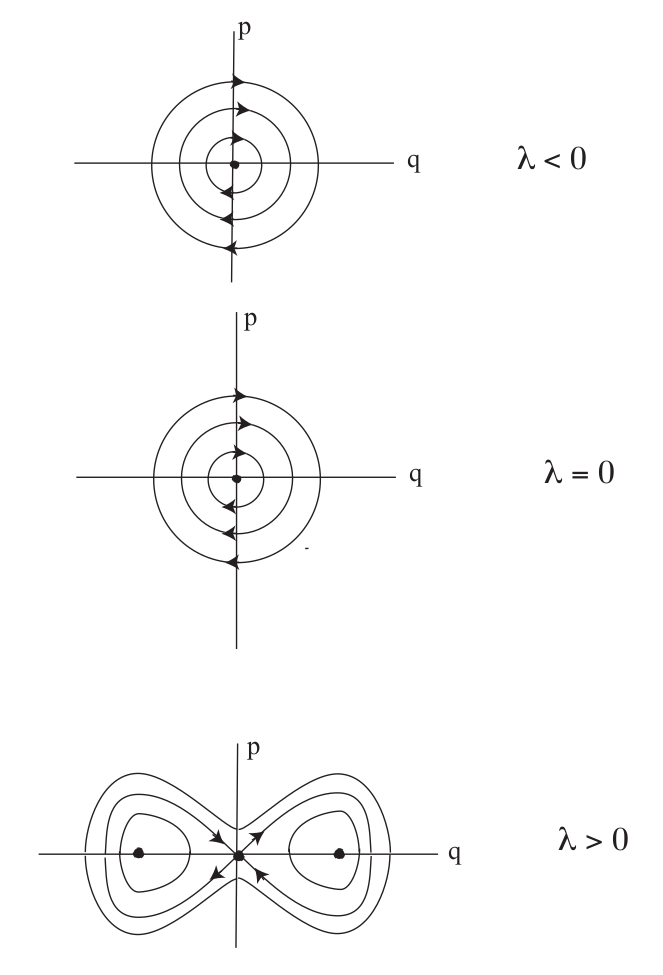
\includegraphics[width=0.6\columnwidth]{ham_pitch.png}
\end{center}
\caption{The phase portraits for the Hamiltonian pitchfork bifurcation.}
\label{fig:appC_fig4}
\end{figure}










\end{document}


